\documentclass{article}
\PassOptionsToPackage{numbers,sort&compress}{natbib}
\usepackage[nonanonymous]{neurips_2026}
\usepackage[utf8]{inputenc}
\usepackage[T1]{fontenc}
\usepackage{hyperref}
\usepackage{url}
\usepackage{booktabs}
\usepackage{amsfonts}
\usepackage{amsmath}
\usepackage{microtype}
\usepackage{xcolor}
\usepackage{graphicx}
\usepackage{tikz}
\usetikzlibrary{positioning,arrows.meta}
\hypersetup{hidelinks}
% Suppress the conference notice; number the first page like the later pages (as in the midpoint report).
\makeatletter
\renewcommand{\@notice}{}
\makeatother
\newcommand{\ci}[2]{[$#1$,\,$#2$]}
\title{Learning to Select Context per Code Diff:\\An Accuracy--Cost Trade-off for LLM Code Review}
\author{Michael Liu (msl196) \quad Ruiding Feng (rf711) \quad Li-Hua Peng (lp880)\\
Machine Learning II, Rutgers University}
\begin{document}
\nolinenumbers
\maketitle
\thispagestyle{plain}
\begin{abstract}
An LLM can review a code change from the diff alone or with surrounding repository code, and every added piece of context costs input tokens. We ask whether a small selector can choose the context for each change so that a frozen reviewer keeps its quality at a lower cost. We build an offline outcome table on all 185 buildable pull requests of AACR-Bench: one reviewer (Qwen3.8-27B) reviews each of 1,811 diff hunks at four context levels, and a judge matches its findings to 1,419 reference comments. No fixed level covers more reference comments than no context (52.3\% to 53.2\%), although wider levels cost 1.3 to 2.2 times as much. Eleven selectors, from logistic regression on hand-made features to an untrained 7B code model, rank the hunks that gain from context at AUC 0.48 to 0.58, and none beats random choice at an equal token budget. Yet the choice matters hunk by hunk: a third of the comments are covered at some levels only, and a selector with hindsight would cover 17\% more comments for 8\% more cost. One request per hunk also covers over a third more comments than an agentic harness on the same model, at 5\% to 11\% of its cost. The trade-off we set out to learn exists; the signal that predicts it is still missing.
\end{abstract}
\noindent\textbf{Repository:} \url{https://github.com/michaelsliu3/CS536_Project}

\section{Introduction}
LLM code review tools must decide how much of a repository to show the model. A diff can be self-contained, or it can only be judged with the function it sits in, the rest of the file, or the code it calls. Agentic harnesses resolve this by letting the model ask: it runs searches and reads files over many requests, and each request resends the growing conversation. That is costly, and context that is not needed can also mislead a model \citep{shi2023distracted}. The alternative we study decides \emph{before} the review which context a change needs, and then makes one request.

\paragraph{Research question.} We ask: \emph{can a small learned selector choose context separately for each code change, so that a frozen LLM reviewer keeps its review quality while using fewer input tokens than fixed context choices?} A positive answer would match the best fixed choice with clearly fewer context tokens, or do better at an equal budget. A negative answer would leave the accuracy--cost curve where fixed choices put it, and would then owe an account of when context helps or harms. We split this into three questions, which organize the report: how much fixed context choices change quality and cost (RQ1), whether a learned selector improves the accuracy--cost frontier over the best fixed choice (RQ2), and when context helps, does nothing, or hurts, and where the selector fails (RQ3).

\paragraph{An earlier pilot and the design it led to.} We first tested the question on ContextCRBench \citep{hu2025contextcrbench}, fine-tuning a 3B reviewer to predict whether a change was merged. The adapter predicted the majority class for every example: 87.5\% accuracy, macro-F1 0.467 and a within-repository AUROC of 0.52. Merge status turned out to be a poor proxy for review quality, and accuracy alone hid the failure. Three design decisions follow from that pilot. First, the target is the review itself: we use AACR-Bench \citep{zhang2026aacr}, whose pull requests carry reference review comments, and score a review by the reference comments it covers. Second, the unit of context is a nested \emph{level} built from a code graph of the repository, in place of issue and pull-request text fields. Third, the reviewer is a larger frozen model, so that the only learned component is the small selector. We built the whole pipeline end to end in its simplest form and then changed one part at a time, which is how the experiments below are ordered.

\paragraph{Findings.} The main result is negative for the selector as built and positive for its premise.
\begin{itemize}
\item \textbf{RQ1.} On all 185 pull requests no fixed context level covers more reference comments than no context. A gain seen on the first 93 pull requests did not repeat on the other 92.
\item \textbf{RQ2.} No selector we trained or prompted beats random choice at an equal token budget. A priced feedback loop that reviews a few hunks again adds comments, at a rising cost per comment, and is matched by a rule that re-reviews the largest hunks.
\item \textbf{The premise holds.} Context decides \emph{which} comments are found for a third of them, and a selector with hindsight would add 17\% more comments for 8\% more cost. One request per hunk covers more than an agentic harness on the same model at about one twentieth of the cost.
\item \textbf{RQ3.} More context changes which problem the reviewer mentions and how it words it, not how many it finds, and the signal our selectors do pick up is mostly the size of the hunk.
\end{itemize}

\section{Related work}
CodeReviewer \citep{li2022codereviewer} pre-trains models for review tasks on diffs without repository context. ContextCRBench \citep{hu2025contextcrbench} adds issue, pull-request and surrounding-code context and compares fixed combinations; our pilot used it. AACR-Bench \citep{zhang2026aacr} provides repository-level reference comments and reports plain LLMs reviewing one diff hunk per request; we use its data, prompt and scoring rule. Selecting context is studied mostly outside review: Repoformer \citep{wu2024repoformer} learns when retrieval is worth adding for code completion, and RECOMP \citep{xu2023recomp} selects or compresses retrieved text for language models. Irrelevant context is known to lower accuracy on reasoning problems \citep{shi2023distracted}. We do not claim that context selection is new. Our contribution is an evaluation: whether per-change selection beats well-chosen fixed policies for code review when the selector is a separate small model, with every token counted and an agentic harness \citep{openai2026codex} as the reference point.

\section{Method}
\begin{figure}[t]
\centering
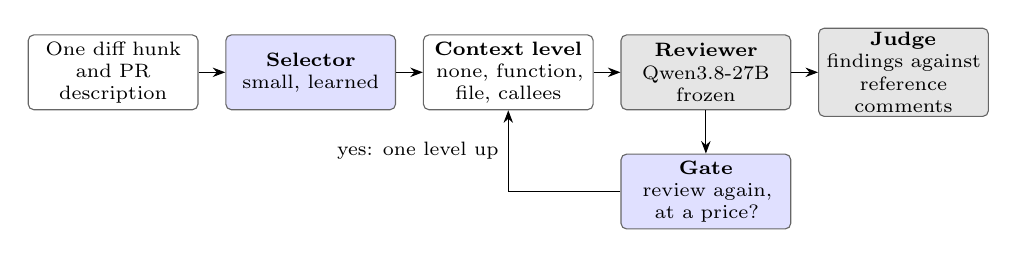
\begin{tikzpicture}[font=\scriptsize, node distance=3.4mm, >={Stealth[length=1.6mm]},
  box/.style={draw=black!60, rounded corners=2pt, minimum height=9.5mm, text width=20.5mm, align=center, inner sep=1.5pt},
  learn/.style={box, fill=blue!12}, frozen/.style={box, fill=black!10}]
\node[box] (hunk) {One diff hunk\\and PR description};
\node[learn, right=of hunk] (sel) {\textbf{Selector}\\small, learned};
\node[box, right=of sel] (ctx) {\textbf{Context level}\\none, function, file, callees};
\node[frozen, right=of ctx] (rev) {\textbf{Reviewer}\\\mbox{Qwen3.8-27B}\\frozen};
\node[frozen, right=of rev] (judge) {\textbf{Judge}\\findings against reference comments};
\node[learn, below=5.5mm of rev] (gate) {\textbf{Gate}\\review again, at a price?};
\draw[->] (hunk) -- (sel);
\draw[->] (sel) -- (ctx);
\draw[->] (ctx) -- (rev);
\draw[->] (rev) -- (judge);
\draw[->] (rev) -- (gate);
\draw[->] (gate) -| node[pos=0.75, left] {yes: one level up} (ctx);
\end{tikzpicture}
\caption{The system. The reviewer and judge are frozen; the selector and the gate are the only learned parts. The reviewer and judge are run once for every hunk at every level, and that offline outcome table is what the selectors and the gate are trained and evaluated on.}
\label{fig:system}
\end{figure}

\paragraph{Data.} AACR-Bench \citep{zhang2026aacr} has 196 pull-request records; 185 can still be built at the reviewed commit, from 50 repositories in ten languages. A \emph{hunk} is one block of the diff with three unchanged lines around each change. We review every hunk in a file that has a reference comment: 1,812 hunks, of which one exceeds the reviewer's 256,000-token input limit. The 185 pull requests carry 1,419 reference comments, 362 written by people and 1,057 generated by AI review tools and verified by the benchmark's annotators. The reviewer model, with its thinking mode on, labelled each comment's severity (94 blocking, 393 should fix, 923 nit, 9 unreadable).

\paragraph{Context levels.} For each repository we build a static code graph with Codebase-Memory \citep{vogel2026codebasememory}, which uses tree-sitter parsers and no LLM. From the graph, each hunk gets four nested inputs: \emph{no context} (the pull request's title and description and the hunk), the enclosing \emph{function} or class, the \emph{file}, and the definitions of the hunk's direct \emph{callees}. We began with ten levels that went on to callers, tests, repository guide files and two-hop neighbours. A pilot on 28 pull requests, read row by row before any larger run, showed every level past the direct neighbours covering fewer comments than no context at 19 to 41 times its tokens, so four levels were kept.

\paragraph{Reviewer and judge.} The reviewer is Qwen3.8-27B \citep{qwen38} served with vLLM \citep{kwon2023vllm} on one GPU, with thinking off. It receives the benchmark's own prompt for non-agent methods, once per hunk, and must quote the lines each finding is about; only findings that quote the reviewed hunk are counted. The same model, in a separate request, judges whether a finding and a reference comment on the same file describe the same issue. This is a similarity decision and not a correctness decision, so the judge does not need to be a better reviewer than the reviewer. Our first table used one request per pull request and a prompt that preferred silence over a doubtful finding; it covered 6 to 7\% of the reference comments at every level. One request per hunk with the benchmark's prompt covers about half, and everything below uses it.

\paragraph{Outcome table and metrics.} Every hunk is reviewed and judged at every level once (7,244 reviews). \emph{Recall} is the share of the 1,419 reference comments covered by some counted finding, and \emph{precision} the share of findings that match a reference comment. A \emph{severity score} is recall weighted by 5, 2 and 0.5 for blocking, should-fix and nit comments. \emph{Cost} is the input and output tokens the model server counted, priced at \$2 and \$10 per million; nothing was billed, and the price only fixes the exchange rate between input and output. Intervals are the middle 95\% of bootstrap draws that resample whole repositories. Because the table is computed offline, a selector or a loop is evaluated by lookup, without new reviews.

\paragraph{Selectors.} Every hunk is reviewed with no context, and a selector ranks the hunks to upgrade to a wider level until a token budget is spent. A hunk is \emph{positive} when some wider level covers more reference comments than no context: 337 of 1,811 hunks. Selectors see only what is known before any review. We keep the benchmark's issue category and context label out of their inputs: both are annotations of the answer, and a selector could learn the category in place of the code. Three families are compared on five folds of whole repositories, with every score out of fold. (i) \emph{Hunk facts}: 71 hand-made features (sizes, counts from the code graph, language, kind of path, tokens each level would add) with a logistic regression, kept as the interpretable baseline, and with random forests and boosted trees. (ii) \emph{Text}: TF-IDF of the path and the hunk, and a language-only control. (iii) \emph{Code models}: Qwen2.5-Coder \citep{hui2024qwencoder} at 1.5B, 3B and 7B, asked whether more code would help the reviewer and scored by $\log P(\text{Yes})-\log P(\text{No})$ with no training; on the first 93 pull requests also a 14B model, frozen embeddings with a linear head, and LoRA fine-tuning \citep{hu2021lora} with three seeds. Baselines are each fixed level, random choice (1,000 orders, whose 95th percentile a selector must beat), cheapest hunks first, and a hindsight choice that knows each outcome.

\paragraph{A priced feedback loop.} One shot may not always be enough, so we also let a hunk ask for more at a price. After a review, a \emph{gate} scores the chance that the next level would cover a comment the reviews so far missed. If the score reaches the price, the hunk is reviewed again one level up, the findings of all its reviews are kept, and every request is paid in full. The gate is a logistic regression per step on 29 facts known before the review and 7 facts of the review just made, trained out of fold; we also tried the 7B code model as the gate, asked after reading the review. The loop is simulated on the saved reviews.

\paragraph{The agentic reference.} To measure what an agentic loop costs, we ran Codex CLI \citep{openai2026codex} on the same served model: one session per hunk, given our reviewer's request, free to search and read the checked-out repository, with a 15-minute limit. Its reviews are scored exactly like ours. Hunks were run in a fixed random order and the run was stopped at 1,000, so these are a random sample of the 1,811.

\section{Experiments and results}
\subsection{RQ1: fixed context levels}
\begin{table}[t]
\caption{The four fixed levels. Recall is the share of reference comments covered. On all 185 pull requests no level beats no context, and the gain on the first 93 is absent on the new 92.}
\label{tab:levels}
\centering
\small
\setlength{\tabcolsep}{4pt}
\begin{tabular}{lrrrrrcrr}
\toprule
 & Input tokens & & \multicolumn{3}{c}{Recall (\%)} & Change from none, & Precision & Severity\\
\cmidrule(lr){4-6}
Level & per PR & Cost & First 93 & New 92 & All 185 & all 185 (points) & (\%) & score\\
\midrule
No context & 9,510 & 1.00 & 50.0 & 54.4 & 52.3 & & 24.4 & 0.578\\
Function & 15,482 & 1.32 & 53.1 & 53.1 & 53.1 & $+0.8$ \ci{-1.5}{+2.9} & 25.3 & 0.589\\
File & 23,964 & 1.73 & 52.2 & 52.4 & 52.3 & $\phantom{+}0.0$ \ci{-2.7}{+2.8} & 25.1 & 0.597\\
Callees & 35,796 & 2.17 & 52.0 & 54.3 & 53.2 & $+0.9$ \ci{-1.3}{+3.1} & 25.0 & 0.599\\
\bottomrule
\end{tabular}
\end{table}

\begin{figure}[t]
\centering
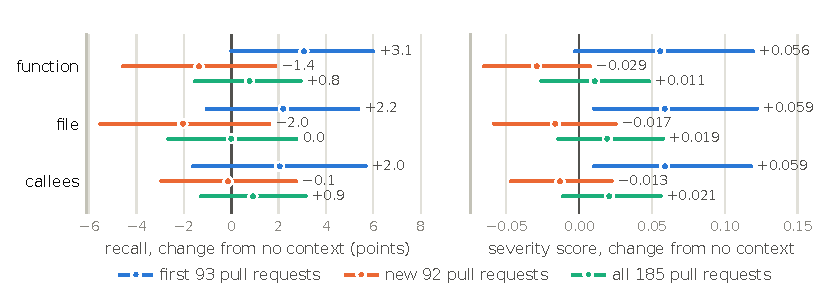
\includegraphics[width=\textwidth]{figures/levels.pdf}
\caption{Each wider level against no context, with 95\% intervals over repositories. The first half suggested a gain from context; the second half, run with the comparisons fixed in advance, did not confirm it.}
\label{fig:levels}
\end{figure}

We scaled the table in steps: 28 pull requests, then 93, then the remaining 92. On the first 93, context looked useful: the function level added 3.1 points of recall and the wider levels about 0.06 of severity score (Table~\ref{tab:levels}, Figure~\ref{fig:levels}). An analysis of that half by groups of comments found two places where levels seemed to differ, and we wrote both down as comparisons before the other 92 pull requests were built. Neither was confirmed. Blocking comments had been covered 15.8 points more often with context \ci{+2.7}{+32.3}; on the new half the change is $-3.6$ \ci{-12.1}{+4.6}. Comments the benchmark marks as needing the repository gained 9.3 points from the file level over the function level; on the new half the gain is $+3.2$ \ci{-5.6}{+12.5}.

On all 185 pull requests the four levels are within 13 covered comments of each other out of 1,419, and every interval for a wider level against no context includes zero, for recall and for the severity score under five weightings. Precision is 24 to 25\% at every level. Wider levels cost 1.3 to 2.2 times as much, so \emph{no context is the best fixed choice}. We report each result for all comments and separately by who wrote them: comments written by people are covered less often than AI-generated ones at every level (43 to 45\% against 55 to 56\%), and neither group gains from context beyond chance.

\subsection{RQ2: learned selectors}
\begin{table}[t]
\caption{Selectors on all 185 pull requests, out of fold. AUC is for ranking the 337 hunks that gain from context. The budget columns upgrade hunks to the function level until 30\% of that level's extra tokens are spent (cost 1.08). No selector exceeds the 95th percentile of random choice.}
\label{tab:selectors}
\centering
\small
\setlength{\tabcolsep}{4.5pt}
\begin{tabular}{lcrr}
\toprule
Selector & AUC [95\% interval] & Covered & Severity score\\
\midrule
Qwen2.5-Coder 7B, asked directly (untrained) & 0.576 \ci{0.542}{0.616} & 759 & 0.594\\
Qwen2.5-Coder 3B, asked directly & 0.565 \ci{0.533}{0.601} & 750 & 0.581\\
Qwen2.5-Coder 1.5B, asked directly & 0.552 \ci{0.510}{0.587} & 740 & 0.569\\
Hunk facts, random forest & 0.553 \ci{0.524}{0.580} & 750 & 0.582\\
Hunk facts, logistic regression & 0.545 \ci{0.512}{0.579} & 739 & 0.577\\
Hunk text (TF-IDF), logistic regression & 0.541 \ci{0.500}{0.584} & 744 & 0.574\\
Language only, logistic regression (control) & 0.481 \ci{0.440}{0.524} & 737 & 0.576\\
\midrule
Random choice: average (95th percentile) & 0.5 & 751.6 (765) & 0.586 (0.599)\\
Cheapest hunks first, no learning & 0.440 \ci{0.399}{0.475} & 758 & 0.594\\
No context for every hunk (cost 1.00) & & 742 & 0.578\\
Function level for every hunk (cost 1.32) & & 753 & 0.589\\
Hindsight choice (knows each outcome) & & 865 & 0.677\\
\bottomrule
\end{tabular}
\end{table}

Table~\ref{tab:selectors} gives the selectors that were run on all 185 pull requests. Their ranking of the hunks that gain from context is weak: AUC 0.48 to 0.58 over eleven selectors, where 0.5 is a coin flip (four more variants are in Appendix~\ref{app:results}). The best is the untrained 7B model. At a budget the ranking does not turn into coverage. With 30\% of the function level's extra tokens the 7B model covers 759 comments, against 751.6 on average and 765 at the 95th percentile for random choice; over eleven selectors, three upgrade levels and seven budgets, 2 of 231 points exceed random choice's 95th percentile, fewer than chance would give. The language-only control is at chance, so a selector cannot score by recognizing the kind of repository.

Model capacity and training data are not what is missing. On the first 93 pull requests, where 21 selectors were compared, forests and boosted trees did not beat the linear model on the same facts, adding the hunk's text added 0.001 of AUC, a 14B model matched the 7B one (0.592 against 0.591), frozen embeddings alone did not beat the hand-made facts, and LoRA fine-tuning was the weakest family. The fact-based selector ranks at 0.55 to 0.57 at every training-set size we tried.

The table also shows why the question is still worth asking. The hindsight choice covers 865 comments at the same budget: 17\% more than no context for 8\% more cost, and far above the 753 that the function level reaches for every hunk at 32\% more cost. A per-hunk choice of context is worth a great deal; we have not yet found inputs that predict it.

\subsection{A priced feedback loop}
\begin{figure}[t]
\centering
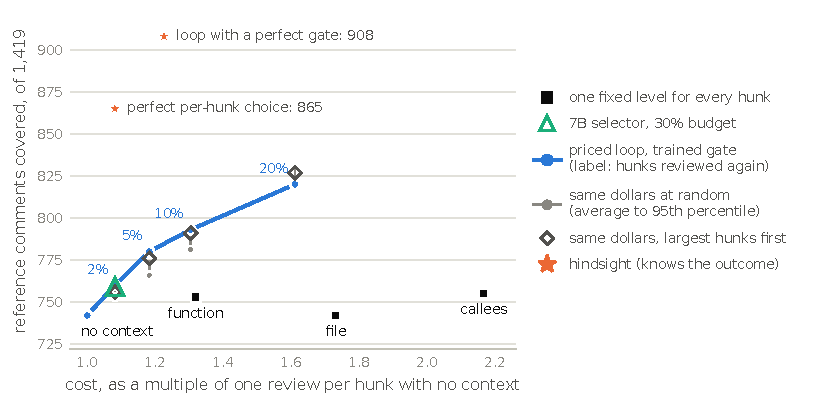
\includegraphics[width=\textwidth]{figures/frontier.pdf}
\caption{The accuracy--cost trade-off on all 185 pull requests. Fixed levels move right without moving up. The loop moves up at a price, level with re-reviewing the largest hunks. The two hindsight policies show the room a better predictor would have.}
\label{fig:frontier}
\end{figure}

The loop keeps the one-shot design and lets a few hunks ask again (Figure~\ref{fig:frontier}). At the price that sends 2\% of hunks back, it covers 760 comments at 1.08 times the cost of one review per hunk; at 5\%, 10\% and 20\% it covers 780, 793 and 820 at 1.18, 1.30 and 1.61 times the cost. It beats the function level for every hunk at a lower cost (780 at 1.18 against 753 at 1.32), because the loop keeps the first review's findings and a wider level replaces them. Each extra comment costs 3.4 to 5.8 times what a first-pass comment costs.

Whether the gate earns its place is a separate question, and we test it at equal cost. Up to a tenth of the hunks, the same dollars spent on second reviews of random hunks do as well in only 1 to 4\% of draws. But spending them on the largest hunks first, with no gate and no training, comes within 2 to 4 comments. The gate ranks the hunks that gain at AUC 0.642 \ci{0.603}{0.675} on the first step, and 0.628 of that comes from facts known before the review; what the first review says adds little. A gate that knew the answer would cover 908 comments at 1.23 times the cost. Asking the 7B code model to be the gate, after it reads the hunk and the review, does not work. It is at chance on the first two steps (AUC 0.518 \ci{0.477}{0.555} and 0.483 \ci{0.423}{0.541}), it answers yes for 62\% of hunks on the first step whether or not a second review pays off, and its loop covers no more than the same dollars spent on random hunks (Appendix~\ref{app:results}). Letting the selector choose the starting level and then running the loop does about the same at equal cost as starting every hunk with no context (Appendix~\ref{app:results}).

\subsection{The cost of an agentic harness}
\begin{table}[t]
\caption{Codex CLI against our one-request reviews on the same model and the same 1,000 randomly ordered hunks. Covered counts the reference comments matched by the reviews of these hunks.}
\label{tab:codex}
\centering
\small
\setlength{\tabcolsep}{4pt}
\begin{tabular}{lrrrrrc}
\toprule
 & Requests & Input tokens & Total & Comments & Findings & Codex minus this row\\
Reviewer & per hunk & per hunk & cost (\$) & covered & off the hunk & [95\% interval]\\
\midrule
Codex CLI, agentic & 16.3 & 348,720 & 114.21 & 415 & 2,197 & \\
Ours, no context & 1 & 958 & 5.87 & 568 & 25 & $-153$ \ci{-226}{-86}\\
Ours, function & 1 & 1,547 & 7.56 & 578 & 128 & $-163$ \ci{-238}{-100}\\
Ours, file & 1 & 2,425 & 9.98 & 572 & 257 & $-157$ \ci{-231}{-88}\\
Ours, callees & 1 & 3,601 & 12.47 & 569 & 276 & $-154$ \ci{-219}{-93}\\
\bottomrule
\end{tabular}
\end{table}

Table~\ref{tab:codex} measures the alternative to selecting context in advance. On 1,000 hunks Codex makes 16.3 requests per hunk and reads 348,720 input tokens, because every request resends its instructions and the conversation so far. Even with cached input priced at a twentieth of new input, it costs 19.4 times our no-context review and 9.2 times our widest level. It also covers fewer of the reference comments: 415 against 568 to 578, a difference of 27 to 28\% whose interval excludes zero for every level. Codex writes 2,197 findings about code outside the hunk it was asked to review, which the scoring does not count; its exploration draws it away from the change. The gap is not uniform. A split made after seeing the totals shows Codex behind on comments answerable from the diff or the file (182 against 242, and 109 against 152 with no context) and level with our reviews on comments that need the repository (64 against 63 to 74): exploring buys parity where the repository is needed and loses elsewhere. For this reviewer and benchmark, one request with context chosen in advance is the stronger and far cheaper design, which is the premise of a selector.

\section{Observations: when context helps, and why the selectors fail}
\paragraph{Context changes which comments are found, not how many.} The reviewer writes about 1.5 findings per hunk at every level (2,708 to 2,772 findings on 1,811 hunks). Of the 1,419 reference comments, 505 are covered at all four levels, 424 at none, and 490 (34.5\%) at some levels and not others. From no context to the function level 179 hunks cover more and 181 cover fewer. The levels average the same because each wider level loses about as many comments as it gains.

\paragraph{More context pulls attention off the change.} Findings that quote code outside the reviewed hunk rise from 25 with no context to 276 with callees on the 1,000-hunk sample of Table~\ref{tab:codex}. On comments the benchmark marks as answerable from the diff, the file level covers 4.6 points fewer than the function level \ci{-7.7}{-1.0}, a difference seen on the first half and repeated on the second. In the ten-level pilot the widest levels fell below no context. This is the behaviour reported for irrelevant context on other tasks \citep{shi2023distracted}, and it means unneeded context is not only a token cost.

\paragraph{The wording does change.} Comparing the reviews across levels directly, with no reference comments involved, shows a difference that holds on both halves of the data: with no context 52\% of findings ask the author to check something and with callees 41\% do, a change of $-11.5$ points \ci{-14.8}{-8.6}; findings that say code cannot be seen fall from 10\% to 6\%. Context makes the reviewer more definite without making it cover more.

\paragraph{Why prediction is hard.} Two measurements bound what any selector can do here. First, the label is noisy: on five pull requests reviewed three times, one level run twice disagrees on 6.1\% of comments, against 15.2\% for two different levels on the same pull requests, so a good part of ``this hunk needs context'' is run-to-run variation. Second, the usable signal is mostly size. The 7B model answers yes for 86\% of hunks that carry a blocking comment against 72\% of the others, a difference of 14.1 points \ci{+7.0}{+20.4}, but the number of changed lines alone ranks those hunks better (AUC 0.688 against 0.625), and the loop's gate is matched by a largest-first rule.

\section{Lessons learned}
\textbf{Run the whole pipeline first.} The largest effect in the project was not context. It was the unit of review and the reviewer's prompt, found only once every stage ran end to end: moving from one request per pull request to one per hunk raised recall from about 6\% to about 52\%.
\textbf{Confirm on new data.} The gain on blocking comments was the largest of 18 groups we had looked at, and it vanished on the second half. Writing the comparison down before the second run is what let us call it chance.
\textbf{Do not trust a proxy or a single number.} Merge status in the pilot, and accuracy on an imbalanced label, both looked fine while the model had learned nothing; we report ranking metrics with intervals over repositories.
\textbf{Price the trivial baselines.} Random choice at an equal budget and a size rule were the comparisons that decided every claim about selectors and the gate.
\textbf{Simulate before paying.} The offline table let us test 21 selectors, a loop and its gates without a new review.

\section{Limitations and future work}
This is initial evidence from one benchmark, one reviewer model and one judge. The judge is the reviewer's own model and no person has audited its matches or the severity labels; a judge from another model family and a human-checked sample are the first checks to add. Each hunk and level was reviewed once, findings that match no reference comment are not scored, and the loop was simulated from reviews that did not see each other. With 185 pull requests, the later steps of the loop have 145 and 68 positive hunks to learn from.

The results point to specific next steps. The selector needs inputs that are about what a wider level would add, such as whether the hunk calls code defined elsewhere, and not only about the hunk. Fixed levels are coarse: choosing individual items from the code graph is the natural target once a signal exists. The loop should be run with real second reviews that see the first, together with a second review at the \emph{same} level, to separate the value of context from the value of asking twice. And the reviewer's sensitivity to where context sits in the prompt remains untested.

\section{Conclusion}
We set out to learn which context each code change needs. On a full benchmark, with a frozen reviewer, we found that no fixed context level and no learned selector improves on reviewing the diff alone, and that the signals available before a review reduce mostly to the size of the change. The same data shows the target is real: the choice of context decides a third of the comments, a perfect per-hunk choice would add 17\% more for 8\% more cost, and one well-formed request per hunk already beats an agentic harness at a twentieth of its cost. The open problem is the predictor, and the outcome table, loop and baselines built here are the instruments for working on it.

\paragraph{Acknowledgments and use of tools.} We thank Professor Lesia Semenova for feedback throughout the project. We used LLM coding assistants (OpenAI Codex, Cursor and Anthropic's Claude Code) to write and debug code, to run analyses and to edit text. Every number in this report is produced by scripts in the repository from saved model outputs; the team checked the implementation and is responsible for the results. The benchmark, models and tools we build on are cited above.

\paragraph{Team contributions.} Michael Liu: project lead, research design, pipeline and analysis software. Ruiding Feng and Li-Hua Peng: model training, selector experiments, evaluation and report preparation.

\bibliographystyle{plainnat}
\bibliography{references}

\appendix
\section{From the proposal to the final report}
\label{app:plan}
Table~\ref{tab:plan} sets the proposal's plan beside what was done. The research question, the frozen reviewer, the small selector, the baselines and the accuracy--cost evaluation are as proposed. The benchmark, the form of context and the quality measure changed after the midpoint, for the reasons in the introduction. The proposal named two risks that came true: that a fixed choice would be near optimal, and that a selector would learn a size rule. In both cases the fallback it set, an analysis of where context helps and why learning fails, is what Sections 4 and 5 report.

\begin{table}[h]
\caption{The proposal's plan and what the project did.}
\label{tab:plan}
\centering
\small
\begin{tabular}{p{0.12\textwidth}p{0.345\textwidth}p{0.41\textwidth}}
\toprule
 & Proposal & Final\\
\midrule
Question & Per-diff context selection for a frozen reviewer: same quality, fewer tokens & Unchanged\\
Benchmark & ContextCRBench, merge status as the label & AACR-Bench, reference review comments (after the midpoint pilot showed the merge label to be a poor proxy)\\
Context & Four optional fields: issue text, PR text, code before, code after & Four nested levels from a code graph: none, function, file, callees (ten were built, four kept after a pilot)\\
Reviewer & Qwen2.5-Coder 7B, frozen & Qwen3.8-27B, frozen\\
Selector & Compact encoder scoring context chunks & Hand-made facts with linear and tree models; Qwen2.5-Coder 0.5B to 14B asked directly, as frozen embeddings, and with LoRA\\
Quality & Accuracy and macro-F1 on the merge label & Recall and precision against reference comments; severity-weighted recall\\
Baselines & Diff only, all context, best fixed, random, similarity, greedy oracle & Each fixed level, random at an equal budget, cheapest first, hindsight; an agentic harness\\
Added & & A priced feedback loop; the cost of an agentic harness\\
\bottomrule
\end{tabular}
\end{table}

\section{Data, models and reproducibility}
\label{app:setup}
\paragraph{Data.} Of the 196 AACR-Bench records, 11 could not be built because the reviewed commits are no longer available. The 185 built pull requests have 4,136 hunks; the 1,812 in files with a reference comment are reviewed. The first 93 pull requests were drawn at random from a pool of 158; the other 92 are the rest of that pool and 27 mostly very large pull requests it had left out, so the two halves are not exchangeable.

\paragraph{Reviewer, judge and labels.} The reviewer's prompt is the one AACR-Bench prints for non-agent methods, copied without change, with and without a context section; the reply uses the benchmark's tag format. A reply cut off at the output limit is sent again with a larger limit. Reviews and judgments use thinking off; severity labels use thinking on. The second-half run made 3,011 reviews in 2 h 22 min on one RTX PRO 6000 with eight requests at a time; judging took 48 min and severity labelling about 3 h 20 min.

\paragraph{Selectors.} Folds are built by a deterministic rule on whole repositories. Non-LLM selectors and the 1.5B, 3B and 7B models asked directly ran on a laptop (8.5, 18 and 41 minutes for the three models); embeddings, LoRA and the 14B model ran on an A100. Tree models and LoRA use three seeds, and the bootstrap seeds are fixed in the scripts.

\paragraph{Code.} The repository holds the dataset build, the reviewer and judge runners, the analysis scripts and their tests. \texttt{scripts/analysis/confirmation\_run\_report.py} produces Table~\ref{tab:levels} and Figure~\ref{fig:levels}; \texttt{run\_selector185.py} produces Table~\ref{tab:selectors}; \texttt{selector\_loop.py} and \texttt{selector\_gate\_llm.py} produce the loop results; \texttt{codex\_blocks\_report.py} produces Table~\ref{tab:codex}; and \texttt{paper/final/make\_figures.py} draws the figures. The documents under \texttt{docs/} record each run, including the ones that failed.

\section{Additional results}
\label{app:results}
\begin{table}[h]
\caption{Reference comments covered at the four levels on all 185 pull requests, by group (``label'' is the benchmark's context label). The last column is the mean coverage of the three wider levels minus coverage with no context, in points.}
\label{tab:groups}
\centering
\small
\setlength{\tabcolsep}{4.5pt}
\begin{tabular}{lrrrrrc}
\toprule
Group & Comments & None & Function & File & Callees & Wider minus none\\
\midrule
Blocking & 94 & 59 & 60 & 66 & 63 & $+4.3$ \ci{-3.7}{+13.6}\\
Should fix & 393 & 239 & 245 & 240 & 246 & $+1.2$ \ci{-3.2}{+5.9}\\
Nit & 923 & 440 & 443 & 432 & 443 & $-0.1$ \ci{-3.0}{+2.4}\\
Label: diff level & 717 & 399 & 408 & 375 & 385 & $-1.3$ \ci{-3.9}{+1.5}\\
Label: file level & 481 & 230 & 234 & 243 & 244 & $+2.1$ \ci{-1.4}{+5.6}\\
Label: repository level & 221 & 113 & 111 & 124 & 126 & $+3.3$ \ci{-1.7}{+8.5}\\
Written by a person & 362 & 155 & 163 & 157 & 163 & $+1.7$ \ci{-2.1}{+5.2}\\
Generated by an AI tool & 1,057 & 587 & 590 & 585 & 592 & $+0.2$ \ci{-2.2}{+2.8}\\
\bottomrule
\end{tabular}
\end{table}

\begin{table}[h]
\caption{The ten-level pilot on 28 pull requests (190 reference comments), which decided the four kept levels. Levels past the direct neighbours cover fewer comments than no context.}
\label{tab:ten}
\centering
\small
\begin{tabular}{lrrrr}
\toprule
Level & Covered & Recall (\%) & Severity score & Input tokens per hunk\\
\midrule
No context & 106 & 55.8 & 0.602 & 493\\
Function & 106 & 55.8 & 0.636 & 1,000\\
File & 116 & 61.1 & 0.708 & 1,876\\
Callees & 111 & 58.4 & 0.715 & 2,904\\
Callers & 109 & 57.4 & 0.729 & 4,059\\
Tests & 107 & 56.3 & 0.719 & 4,331\\
Guide files and search hits & 99 & 52.1 & 0.635 & 9,340\\
Two hops & 96 & 50.5 & 0.652 & 11,951\\
Two hops with documentation & 99 & 52.1 & 0.663 & 12,228\\
Everything the tracer finds & 94 & 49.5 & 0.631 & 20,176\\
\bottomrule
\end{tabular}
\end{table}

\begin{table}[h]
\caption{Selector families on the first 93 pull requests (928 hunks, 190 positive), where the wider comparison of 21 selectors was run. AUC with 95\% intervals; the best member of each family is shown.}
\label{tab:families}
\centering
\small
\begin{tabular}{llc}
\toprule
Family & Best member & AUC [95\% interval]\\
\midrule
Code model asked directly & 14B (7B: 0.591) & 0.592 \ci{0.538}{0.640}\\
Frozen embeddings with hunk facts & 7B & 0.573 \ci{0.525}{0.628}\\
Frozen embeddings & 7B & 0.555 \ci{0.491}{0.624}\\
Hunk facts with text & logistic regression & 0.552 \ci{0.499}{0.600}\\
Hunk facts & logistic regression & 0.551 \ci{0.498}{0.600}\\
LoRA fine-tuning & 3B & 0.531 \ci{0.466}{0.605}\\
Language only (control) & logistic regression & 0.488 \ci{0.425}{0.535}\\
\bottomrule
\end{tabular}
\end{table}

\begin{table}[h]
\caption{The priced loop on all 185 pull requests: with the trained gate from both starts, and with the 7B code model as the gate. ``Random'' and ``largest'' spend the loop's extra dollars on one second review of random hunks (average of 500 draws, with the share of draws that do as well as the loop) and of the largest hunks first.}
\label{tab:loop}
\centering
\small
\setlength{\tabcolsep}{4pt}
\begin{tabular}{llrrrrrrr}
\toprule
 & & Hunks & Extra & & & & & \\
Start & Policy & again & reviews & Covered & Cost & Random & As good & Largest\\
\midrule
No context & no loop & 0 & 0 & 742 & 1.00 & & & \\
 & loop, 2\% price & 37 & 40 & 760 & 1.08 & 752.8 & 3\% & 756\\
 & loop, 5\% price & 91 & 109 & 780 & 1.18 & 765.9 & 1\% & 776\\
 & loop, 10\% price & 182 & 218 & 793 & 1.30 & 781.1 & 4\% & 791\\
 & loop, 20\% price & 363 & 491 & 820 & 1.61 & 817.9 & 41\% & 827\\
 & perfect gate (hindsight) & 215 & 233 & 908 & 1.23 & & & \\
 & all four levels, every hunk & 1,811 & 5,433 & 995 & 6.22 & & & \\
\midrule
7B selector & no loop & 0 & 0 & 759 & 1.08 & & & \\
 & loop, 2\% price & 32 & 34 & 773 & 1.15 & 766.5 & 2\% & 771\\
 & loop, 5\% price & 71 & 82 & 785 & 1.22 & 773.4 & 1\% & 783\\
 & loop, 10\% price & 136 & 158 & 798 & 1.31 & 783.0 & $<$1\% & 797\\
 & loop, 20\% price & 293 & 378 & 821 & 1.57 & 808.4 & 2\% & 824\\
\midrule
No context, & loop, 2\% price & 37 & 49 & 746 & 1.04 & 747.0 & 74\% & 749\\
7B model & loop, 5\% price & 91 & 117 & 748 & 1.09 & 753.6 & 98\% & 758\\
as the gate & loop, 10\% price & 182 & 245 & 768 & 1.19 & 766.4 & 39\% & 776\\
 & loop, 20\% price & 363 & 547 & 788 & 1.44 & 797.6 & 95\% & 812\\
\bottomrule
\end{tabular}
\end{table}

\begin{table}[h]
\caption{How well the gate ranks the hunks where the next level adds a covered comment (AUC), by step and by what the gate may read. The last column is the 7B code model asked after it reads the hunk and the review.}
\label{tab:gate}
\centering
\small
\setlength{\tabcolsep}{4.5pt}
\begin{tabular}{lrcrrrc}
\toprule
 & Positive & Trained gate & Facts & Review & Changed & 7B model asked\\
Step & hunks & [95\% interval] & before & output & lines & [95\% interval]\\
\midrule
None, function next & 215 & 0.642 \ci{0.603}{0.675} & 0.628 & 0.603 & 0.581 & 0.518 \ci{0.477}{0.555}\\
Function, file next & 145 & 0.532 \ci{0.466}{0.608} & 0.541 & 0.500 & 0.582 & 0.483 \ci{0.423}{0.541}\\
File, callees next & 68 & 0.719 \ci{0.659}{0.788} & 0.702 & 0.612 & 0.577 & 0.597 \ci{0.545}{0.648}\\
\bottomrule
\end{tabular}
\end{table}

\paragraph{Selectors not shown in Table~\ref{tab:selectors}.} The other four selectors run on all 185 pull requests are hunk facts with text under logistic regression (AUC 0.545), boosted trees on hunk facts (0.536), and boosted trees and a random forest on hunk facts with text (0.532 and 0.526). None exceeds random choice at the main budget.

\paragraph{Wording.} On all 185 pull requests, the share of findings that ask the author to check something is 52.1\%, 48.6\%, 44.5\% and 40.7\% at the four levels; the share that say code cannot be seen is 10.4\%, 7.8\%, 7.1\% and 6.3\%; and the share that point to the given context is 10.0\%, 10.7\%, 13.3\% and 13.9\%. All three trends hold separately on the first 93 and the new 92 pull requests.

\paragraph{Must-fix hunks.} 85 hunks carry a blocking reference comment. At the 30\% budget the 7B model upgrades 41.2\% of them against 26.4\% of other hunks, a difference of 14.8 points \ci{+3.3}{+26.6}. The blocking comments covered do not rise with it: 59 of 94 with no context, 60 under the 7B model's choice, and 60 if exactly the must-fix hunks were upgraded to the function level.
\end{document}
